\documentclass{beamer}
\usepackage[utf8]{inputenc}
\usepackage[T1]{fontenc}
% \usepackage{amscd, amsfonts, amsmath, amssymb, amstext, amsthm, caption, epsfig, fancyhdr, float, graphicx, latexsym, mathtools, multicol, multirow, algorithm, chngcntr}
\usepackage[english, french]{babel}
\usepackage{booktabs}

\usepackage{amsmath,amssymb}
\usepackage{graphicx}
\usepackage{caption}
\usepackage{subfig}
\usepackage{xspace}
\usepackage{fourier}


\usepackage{tikz}
\usetikzlibrary{shapes,arrows}
\usepackage{tkz-graph}
\usetikzlibrary{automata,arrows,positioning,calc}
\usetikzlibrary{positioning}
\usetikzlibrary{fit}
\usetikzlibrary{backgrounds}
\usetikzlibrary{calc}
\usetikzlibrary{shapes}
\usetikzlibrary{mindmap}
\usetikzlibrary{decorations.text}
\usetikzlibrary{snakes}

\usepackage{algorithm}
% \usepackage{algorithmic}
\usepackage{algorithmicx}
\usepackage{listings}
\usepackage{hyperref}
\hypersetup{
    bookmarks=true,         % show bookmarks bar?
    unicode=false,          % non-Latin characters in Acrobat’s bookmarks
    pdftoolbar=true,        % show Acrobat’s toolbar?
    pdfmenubar=true,        % show Acrobat’s menu?
    pdffitwindow=false,     % window fit to page when opened
    pdfstartview={FitH},    % fits the width of the page to the window
    pdftitle={My title},    % title
    pdfauthor={Author},     % author
    pdfsubject={Subject},   % subject of the document
    pdfcreator={Creator},   % creator of the document
    pdfproducer={Producer}, % producer of the document
    pdfkeywords={keyword1, key2, key3}, % list of keywords
    pdfnewwindow=true,      % links in new PDF window
    colorlinks=false,       % false: boxed links; true: colored links
    linkcolor=red,          % color of internal links (change box color with linkbordercolor)
    citecolor=green,        % color of links to bibliography
    filecolor=cyan,         % color of file links
    urlcolor=magenta        % color of external links
}

% \theoremstyle{definition} % insert bellow all blocks you want in normal text
% \newtheorem{definition}{Definition}



% tikzmark command, for shading over items
\newcommand{\tikzmark}[1]{\tikz[overlay,remember picture] \node (#1) {};}
% Define block styles
\tikzstyle{decision} = [diamond, draw, fill=blue!20,
    text width=4.5em, text badly centered, node distance=3cm, inner sep=0pt]
\tikzstyle{block} = [rectangle, draw, fill=blue!20,
    text width=5em, text centered, rounded corners]
\tikzstyle{line} = [draw]
\tikzstyle{cloud} = [draw, ellipse,fill=red!20, node distance=3cm,
    minimum height=2em]

\usepackage[most]{tcolorbox}

\setbeamertemplate{blocks}[rounded][shadow=true] % use rounded blocks with standard beamer shadow


% Distributions.
\newcommand*{\UnifDist}{\mathsf{Unif}}
\newcommand*{\ExpDist}{\mathsf{Exp}}
\newcommand*{\DepExpDist}{\mathsf{DepExp}}
\newcommand*{\GammaDist}{\mathsf{Gamma}}
\newcommand*{\LognormalDist}{\mathsf{LogNorm}}
\newcommand*{\WeibullDist}{\mathsf{Weib}}
\newcommand*{\ParetoDist}{\mathsf{Par}}
\newcommand*{\NormalDist}{\mathsf{Norm}}

\newcommand*{\GeometricDist}{\mathsf{Geom}}
\newcommand*{\NegBinomialDist}{\mathsf{NegBin}}
\newcommand*{\PoissonDist}{\mathsf{Poisson}}
\newcommand*{\BivariatePoissonDist}{\mathsf{BPoisson}}
\newcommand*{\CyclicalPoissonDist}{\mathsf{CPoisson}}

\newcommand*{\iid}{\textbf{iid}\@\xspace}
\newcommand*{\pdf}{\textbf{pdf}\@\xspace}
\newcommand*{\cdf}{\textbf{cdf}\@\xspace}
\newcommand*{\pmf}{\textbf{pmf}\@\xspace}
\newcommand*{\abc}{{\textbf{abc}}\@\xspace}
\newcommand*{\smc}{\textbf{smc}\@\xspace}
\newcommand*{\mcmc}{\textbf{mcmc}\@\xspace}
\newcommand*{\ess}{\textbf{ess}\@\xspace}
\newcommand*{\mle}{\textbf{mle}\@\xspace}
\newcommand*{\bic}{\textbf{bic}\@\xspace}
\newcommand*{\kde}{\textbf{kde}\@\xspace}
\newcommand*{\glm}{\textbf{glm}\@\xspace}
\newcommand*{\xol}{\textbf{xol}\@\xspace}
\newcommand*{\cpu}{\textbf{cpu}\@\xspace}
\newcommand*{\gpu}{\textbf{gpu}\@\xspace}
\newcommand*{\arm}{\textbf{arm}\@\xspace}

\def \si {\sigma}
\def \la {\lambda}
\def \al {\alpha}
% \def\e*{\end{eqnarray*}}
\def \di{\displaystyle}

\def \E{\mathbb E}
\def \N{\mathbb N}
\def \Z{\mathbb Z}
\def \NZ{\mathbb{N}_0}
\def \I{\mathbb I}
\def \w{\widehat}
\def \P {\mathbb P}
\def \V{\mathbb V}


\newcommand{\CL}{\mathbb{C}}
\newcommand{\RL}{\mathbb{R}}
\newcommand{\nat}{{\mathbb N}}
\newcommand{\Laplace}{\mathscr{L}}
\newcommand{\e}{\mathrm{e}}
\newcommand{\ve}{\bm{\mathrm{e}}} % vector e

\renewcommand{\L}{\mathcal{L}} % e.g. L^2 loss.

\newcommand{\ih}{\mathrm{i}}
\newcommand{\oh}{{\mathrm{o}}}
\newcommand{\Oh}{{\mathcal{O}}}
\newcommand{\Exp}{\mathbb{E}}

\newcommand{\Norm}{\mathcal{N}}
\newcommand{\LN}{\mathcal{LN}}
\newcommand{\SLN}{\mathcal{SLN}}

\renewcommand{\Pr}{\mathbb{P}}
\newcommand{\Ind}{\mathbb I}
\newcommand\bfsigma{\bm{\sigma}}
\newcommand\bfSigma{\bm{\Sigma}}
\newcommand\bfLambda{\bm{\Lambda}}
\newcommand{\stimes}{{\times}}
\def \limsup{\underset{n\rightarrow+\infty}{\overline{\lim}}}
\def \liminf{\underset{n\rightarrow+\infty}{\underline{\lim}}}


\AtBeginSection[]
  {
     \begin{frame}<beamer>
     \frametitle{Agenda}
     \tableofcontents[currentsection]
     \end{frame}
  }



% vertical separator macro
\newcommand{\vsep}{
  \column{0.0\textwidth}
    \begin{tikzpicture}
      \draw[very thick,black!10] (0,0) -- (0,7.3);
    \end{tikzpicture}
}
\newcommand\blfootnote[1]{%
  \begingroup
  \renewcommand\thefootnote{}\footnote{#1}%
  \addtocounter{footnote}{-1}%
  \endgroup
}

% More space between lines in align
% \setlength{\mathindent}{0pt}

% Beamer theme
\usetheme{ZMBZFMK}
\usefonttheme[onlysmall]{structurebold}
\mode<presentation>
\setbeamercovered{transparent=10}

% align spacing
\setlength{\jot}{0pt}

\setbeamertemplate{navigation symbols}{}%remove navigation symbols

\title[UCSB Intro]{Blockchain and applications}

\author{Pierre-O. Goffard}
\institute[UNISTRA]{Université de Strasbourg\\
 \texttt{goffard@unistra.fr}
}
\date{Spring Quarter 2024}
% \titlegraphic{\includegraphics[width=2.5cm]{../../Figures/bfs_logo.png}} 
% \titlegraphic{
% 
\includegraphics[width=0.25\textwidth]{../../Figures/DALL-E/WS_UNSW_DEFI.png}
% }
\begin{document}
% \begin{frame}[plain]
%   
\includegraphics[width=\textwidth]{../../Figures/DALL-E/WS_UNSW_DEFI.png}
% \end{frame}
\begin{frame}
  \titlepage
\end{frame}
\begin{frame}{Agenda}
  \tableofcontents
\end{frame}

\section{Introduction}
\begin{frame}{Blockchain}
A data ledger made of a sequence of blocks maintained by a achieving consensus in a Peer-To-Peer network.
\begin{columns}
\begin{column}{0.5\textwidth}
% \small

\begin{itemize}
  \item Decentralized
  \item Public/private
  \item Permissionned/permissionless
  \item Immutable
  \item Incentive compatible
\end{itemize}
\end{column}
\begin{column}{0.5\textwidth}
\begin{center}
\begin{tikzpicture}[-, >=stealth', auto, semithick, node distance=01cm]
\tikzstyle{every edge}=[snake=expanding waves,segment length=1mm,segment angle=10, draw]

\tikzstyle{full node}=[circle, fill=tublue,draw=tublue,thick,text=black,scale=0.8]
\tikzstyle{light node}=[circle, fill=white,draw=tublue,thick,text=black,scale=0.8]
\node[full node]    (1)                     {};
\node[full node]    (2)[above right of=1]         {};
\node[full node]    (3)[above left of=1]         {};
\node[full node]    (4)[below of=1]         {};
\node[full node]    (5)[right of=4]         {};
\node[full node]    (6)[below of=4]         {};
\node[light node]    (7)[left of=1]         {};
\node[light node]    (8)[right of=2]         {};
\node[light node]    (9)[left of=4]         {};
\node[light node]    (10)[above right of=5]         {};
\node[light node]    (11)[ right of=5]         {};
\node[light node]    (12)[ below right of=5]         {};
% \node[light node]    (4)[above of=2]         {};
\path

(1) edge node{} (2)
    edge node{} (3)
    edge node{} (7)
    ;
\path
(5) edge node{} (10)
    edge node{} (11)
    edge node{} (12)
    ;
    \path
(4) edge node{} (5)
    edge node{} (1)
    edge node{} (9)
    edge node{} (6)
    ;
    \path
(2) edge node{} (8)   
    ;
\end{tikzpicture}
\end{center}
\end{column}
\end{columns}

% \vspace{0.2cm}
% We will focus on public blockchain and their associated consensus protocol.
\end{frame}
% \begin{frame}{Blocks}
% A block contains
% \begin{itemize}
%   \item block height/ID
%   \item Time stamp
%   \item hash of the block
%   \item hash of the previous block
%   \item Set of transactions (data stored in the blockchain)
% \end{itemize}
% \begin{center}
% 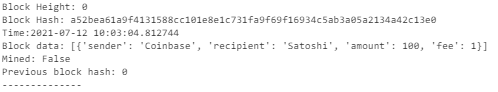
\includegraphics[width=0.9\textwidth]{../../Figures/genesis_block.png}
% \end{center}
% \url{https://www.blockchain.com/}
% \end{frame}

\begin{frame}{Consensus protocols}
The mechanism to make all the nodes agree on a common data history.\\
\vspace{0.3cm}
The three dimensions of blockchain systems analysis
\begin{enumerate}
  \item Efficiency (Queueing theory)
  \begin{itemize}
    \item Throughputs
    \item Transaction confirmation time
  \end{itemize}
  \item Decentralization (Entropy)
  \begin{itemize}
    \item Fair distribution of the accounting right
  \end{itemize}
  \item Security (Insurance Risk Theory)
  \begin{itemize}
    \item Resistance to attacks
  \end{itemize}
\end{enumerate}
\end{frame}

\begin{frame}{Applications of blockchain: Cryptocurrency}
\begin{columns}
\begin{column}{0.5\textwidth}
   
{\footnotesize
\begin{thebibliography}{1}
\bibitem{Na08}
S.~Nakamoto, ``Bitcoin: A peer-to-peer electronic cash system.'' Available at
  \href{https://bitcoin.org/bitcoin.pdf}{https://bitcoin.org/bitcoin.pdf},
  2008.
\end{thebibliography}  
}
\end{column}
\begin{column}{0.5\textwidth}  %%<--- here
    \begin{center}
     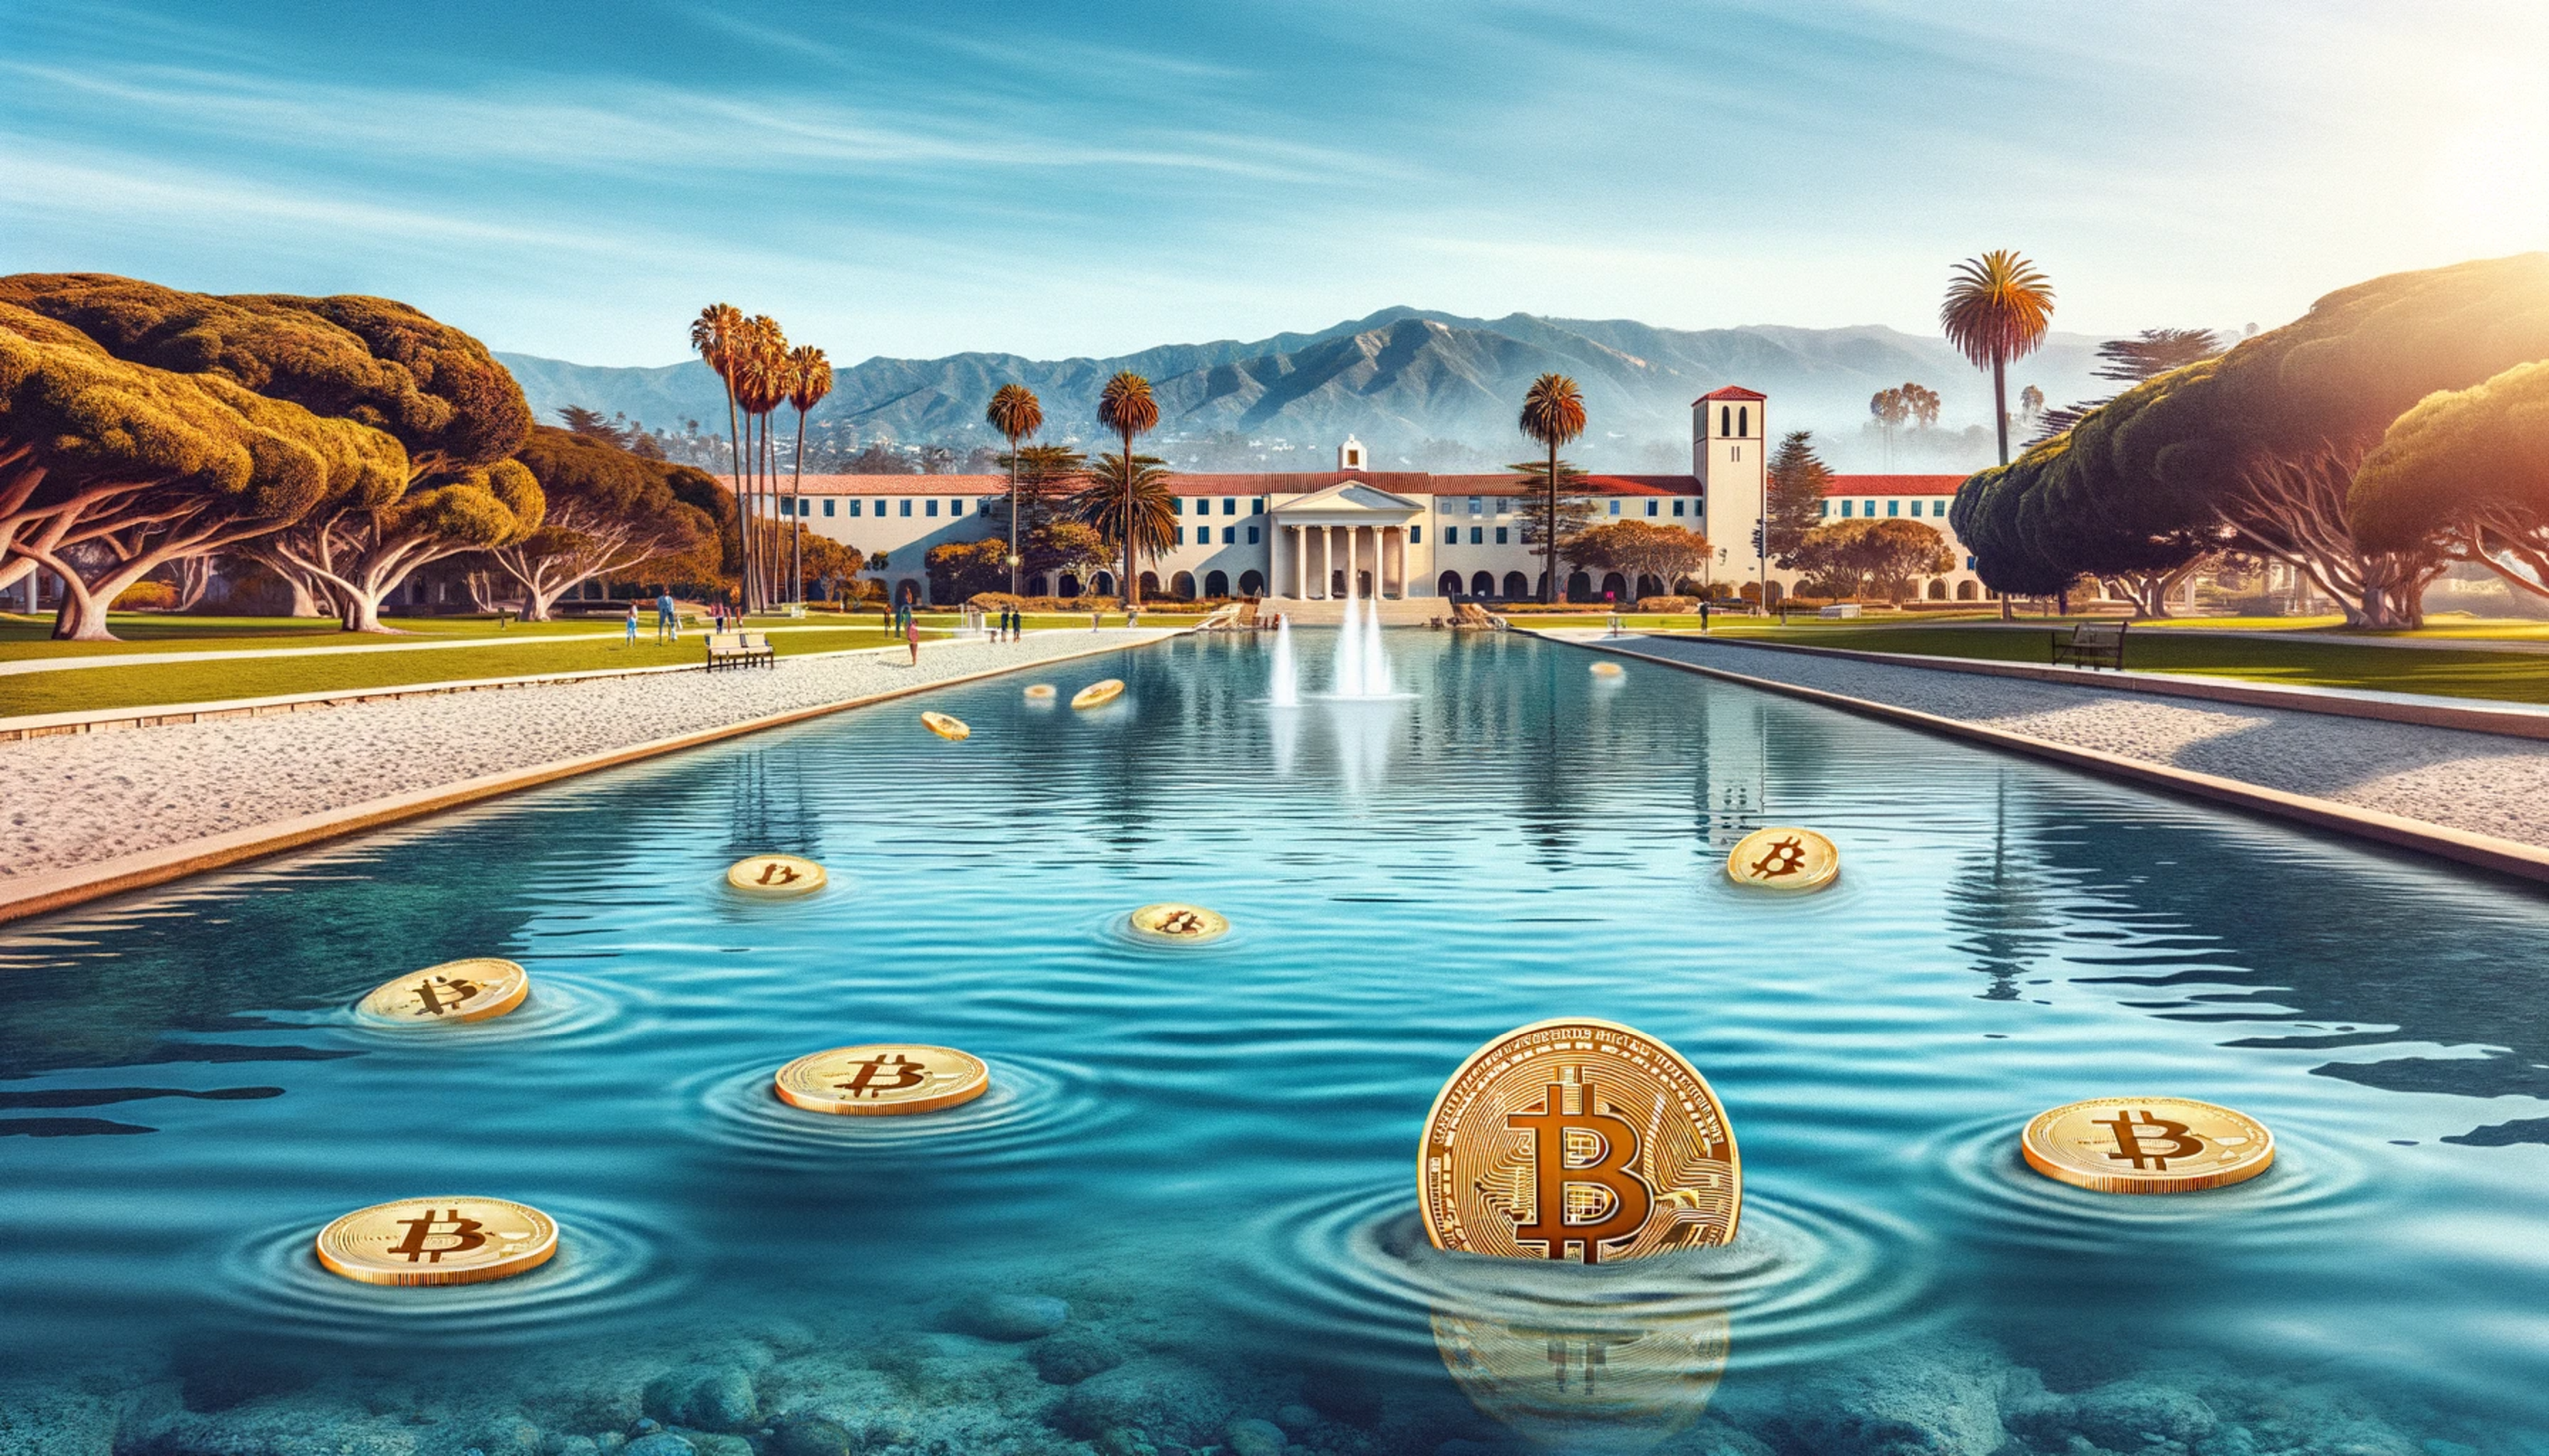
\includegraphics[width=\textwidth]{../../Figures/UCSB_bitcoin}
     \end{center}
\end{column}
\end{columns}
\begin{itemize}
  \item Transaction anonymity
  \item No need for a thrusted third party
\end{itemize}


\end{frame}
\begin{frame}[allowframebreaks]{Reading list}
\scriptsize
\begin{thebibliography}{10}

\bibitem{Li2018}
Q.-L. Li, J.-Y. Ma, and Y.-X. Chang, {\em Blockchain Queue Theory}, pp.~25--40.
\newblock Springer International Publishing, 2018.

\bibitem{Angeris2022}
G.~Angeris, A.~Agrawal, A.~Evans, T.~Chitra, and S.~Boyd, {\em Constant
  Function Market Makers: Multi-asset Trades via Convex Optimization},
  pp.~415--444.
\newblock Springer International Publishing, 2022.

\bibitem{Cartea2023}
A.~Cartea, F.~Drissi, and M.~Monga, ``Execution and statistical arbitrage with
  signals in multiple automated market makers,'' in {\em 2023 IEEE 43rd
  International Conference on Distributed Computing Systems Workshops
  (ICDCSW)}, pp.~37--42, 2023.

\bibitem{Hansjoerg2022OR}
H.~Albrecher and P.-O. Goffard, ``On the profitability of selfish blockchain
  mining under consideration of ruin,'' {\em Operations Research}, vol.~70,
  pp.~179--200, Jan. 2022.

\bibitem{Li2024}
Z.~Li, A.~M. Reppen, and R.~Sircar, ``A mean field games model for
  cryptocurrency mining,'' {\em Management Science}, vol.~70, pp.~2188--2208,
  Apr. 2024.

\bibitem{Bowden2020}
R.~Bowden, H.~P. Keeler, A.~E. Krzesinski, and P.~G. Taylor, ``Modeling and
  analysis of block arrival times in the bitcoin blockchain,'' {\em Stochastic
  Models}, vol.~36, pp.~602--637, July 2020.

\bibitem{Tiwari2019}
A.~K. Tiwari, S.~Kumar, and R.~Pathak, ``Modelling the dynamics of bitcoin and
  litecoin: Garch versus stochastic volatility models,'' {\em Applied
  Economics}, vol.~51, pp.~4073--4082, Mar. 2019.

\bibitem{Dembo2020}
A.~Dembo, S.~Kannan, E.~N. Tas, D.~Tse, P.~Viswanath, X.~Wang, and O.~Zeitouni,
  ``Everything is a race and nakamoto always wins,'' in {\em Proceedings of the
  2020 ACM SIGSAC Conference on Computer and Communications Security}, CCS
  ’20, ACM, Oct. 2020.

\bibitem{Park2023}
A.~Park, ``The conceptual flaws of decentralized automated market making,''
  {\em Management Science}, vol.~69, pp.~6731--6751, Nov. 2023.

\bibitem{Rosu2021}
I.~Roşu and F.~Saleh, ``Evolution of shares in a proof-of-stake
  cryptocurrency,'' {\em Management Science}, vol.~67, pp.~661--672, Feb. 2021.
  
\bibitem{Adams2021}
H.~Adams, N.~Zinsmeister, M.~Salem, R.~Keefer, and D.~Robinson, ``Uniswap v3
  core,'' {\em Tech. rep., Uniswap, Tech. Rep.}, 2021.

\end{thebibliography}
\end{frame}


\section{Consensus protocol}
\begin{frame}{Consensus protocol}
\begin{tcolorbox}[enhanced,drop shadow, title=Definition]
    Algorithm to allows the full nodes to agree on a common data history
\end{tcolorbox}
It must rely on the scarce resources of the network
\begin{itemize}
  \item bandwidth
  \item computational power
  \item storage (disk space)
\end{itemize}
\end{frame}
\begin{frame}{Types of consensus protocols}
\begin{enumerate}
  \item Voting based 
  \footnotesize
\begin{thebibliography}{1}

\bibitem{lamport1982the}
L.~Lamport, R.~Shostak, and M.~Pease, ``The byzantine generals problem,'' {\em
  ACM Transactions on Programming Languages and Systems}, pp.~382--401, July
  1982.

\end{thebibliography}
\normalsize
\begin{itemize}
  \item[\danger] Communication overhead
  \item[\danger] Denial of service
\end{itemize}

  \item Leader based
  \begin{itemize}
    \item Proof-of-Work (computational power)
    \item Proof-of-Capacity and Proof-of-Spacetime (storage)
    \item Proof-of-Interaction (bandwidth)
    \item Proof-of-Stake (tokens)
  \end{itemize}
\end{enumerate}
\end{frame}


\begin{frame}{Proof-of-Work}
\begin{tcolorbox}[enhanced,drop shadow, title=Objective]
    Elect a leader based on computational effort to append the next block.
\end{tcolorbox}
\end{frame}
\begin{frame}{What's inside a block?}
A block consists of 
\begin{itemize}
\item a header 
\item a list of "transactions" that represents the information recorded through the blockchain. 
\end{itemize}
The header usually includes 
\begin{itemize}
\item the date and time of creation of the block, 
\item the block height which is the index inside the blockchain, 
\item the hash of the block 
\item the hash of the previous block. 
\end{itemize}
\begin{tcolorbox}[enhanced,drop shadow, title=Question]
What is the hash of a block?
\end{tcolorbox}
\end{frame}
\begin{frame}{Cryptographic Hash function}
\small
A function that maps data of arbitratry size (message) to a bit array of fixed size (hash value)
$$
h:\{0,1\}^\ast\mapsto \{0,1\}^d. 
$$
A good hash function is
\begin{itemize}
\item deterministic
\item quick to compute
\item One way
\begin{itemize}
  \scriptsize
\item[$\hookrightarrow$] For a given hash value $\overline{h}$ it is hard to find a message $m$ such that 
$$
h(m) = \overline{h}
$$
\end{itemize}
\item Colision resistant 
\begin{itemize}
\item[$\hookrightarrow$] Impossible to find $m_1$ and $m_2$ such that 
$$
h(m_1) = h(m_2)
$$
\end{itemize}
\item Chaotic
$$m_1\approx m_2\Rightarrow  h(m_1) \neq h(m_2)$$
\end{itemize}
\end{frame}
\begin{frame}{SHA-256}
The SHA-256 function which converts any message into a hash value of $256$ bits.
\begin{tcolorbox}[enhanced,drop shadow, title=Example]
The hexadecimal digest of the message
$$
\texttt{Is DeFi the future?}
$$
is 
\footnotesize
$$
\texttt{60a147c28568dc925c347bce20c910ef90f3774e2501ac63344f3411b6a6bf79}
$$
\end{tcolorbox}
\end{frame}
\begin{frame}{Hidden prediction}
\begin{center}
 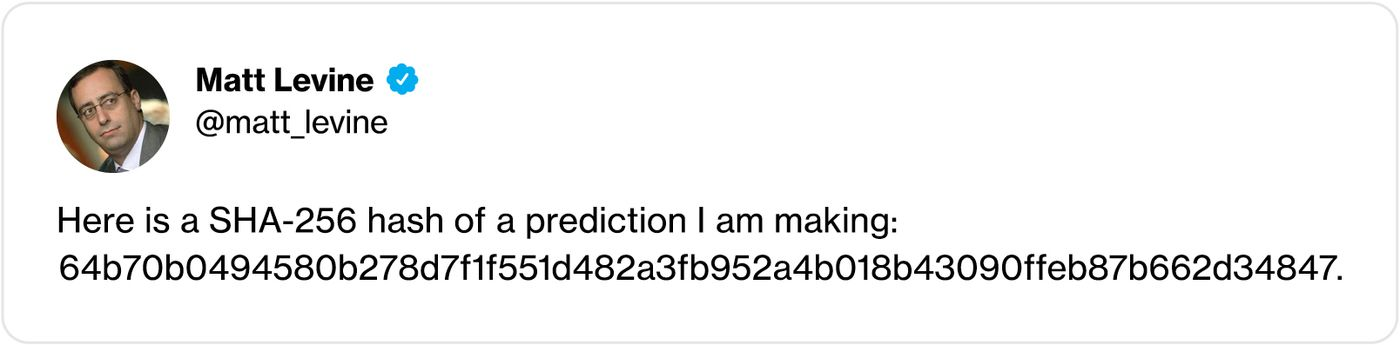
\includegraphics[width= \textwidth]{../../Figures/levine_twitter}
\end{center}
\footnotesize{
\begin{thebibliography}{1}
\bibitem{levine}
M.~Levine, ``The crypto story.'' Bloomberg business week, Oct. 2022.\\
\end{thebibliography}  
}




\end{frame}
\begin{frame}{Mining a block}
\begin{figure}[!ht]
    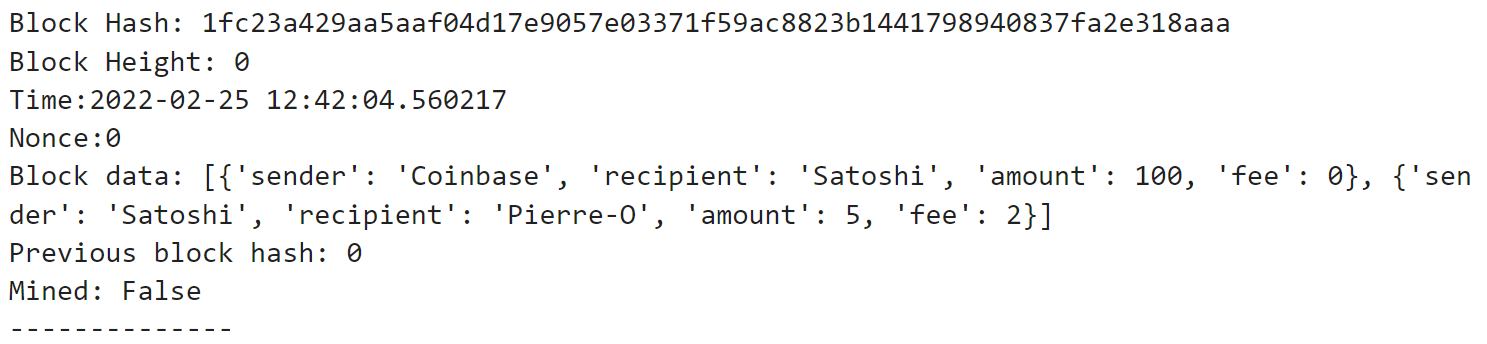
\includegraphics[width = \textwidth]{../../Figures/block_not_mined.png}
    \captionsetup{width=0.8\textwidth}
    \centering
    \caption{A block that has not been mined yet.}
    \label{fig:block_not_mined}
\end{figure}
\end{frame}
\begin{frame}{Mining a block}
The maximum value for a 256 bits number is
$$
T_\text{max} = 2^{256}-1 \approx 1.16e^{77}.
$$
Mining consists in drawing at random a nonce 
$$
\text{Nonce} \sim \text{Unif}(\{0,\ldots, 2^{32}-1\}),
$$
until 
$$
h(\text{Nonce}|\text{Block info})<T,
$$
where $T$ is referred to as the target.
\begin{tcolorbox}[enhanced,drop shadow, title=Difficulty of the cryptopuzzle]
$$
D = \frac{T_{\max}}{T}.
$$
\end{tcolorbox}
\url{https://laub.au/mine/}
\end{frame}
\begin{frame}{Mining a block}
If we set the difficulty to $D = 2^4$ then the hexadecimal digest must start with at least $1$ leading $0$
\begin{figure}[!ht]
    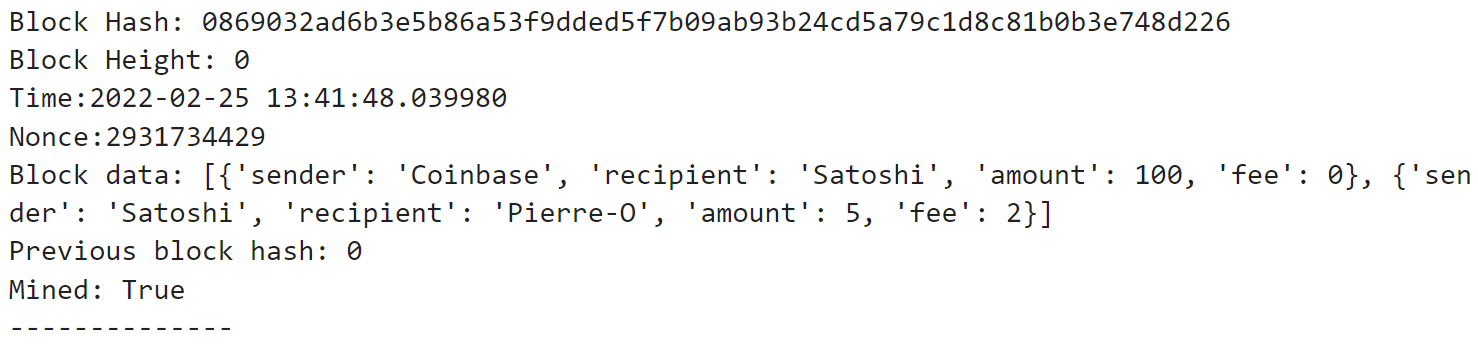
\includegraphics[width = \textwidth]{../../Figures/block_mined.png}
    \captionsetup{width=0.8\textwidth}
    \centering
    \caption{A mined block with a hash value having on leading zero.}
    \label{fig:block_mined}
\end{figure}
The number of trial is geometrically distributed
\begin{itemize}
\item Exponential inter-block times
\item Lenght of the blockchain = Poisson process\blfootnote{\href{https://www.blockchain.com/explorer/blocks/btc/0000000000000000000954d42e8ced7017448cb9f39b364e371a1eec6e34463b}{block info}}
\end{itemize}
\end{frame}
% \begin{frame}{Bitcoin protocol}
% \begin{itemize}
%   \item One block every 10 minutes on average
%   \item Depends on the hashrate of the network
%   \item Difficulty adjustment every 2,016 blocks ($\approx$ two weeks)
%   \item Reward halving every 210,000 blocks
% \end{itemize}
% Check out \url{https://www.bitcoinblockhalf.com/}
% \end{frame}
\begin{frame}{Conflict resolution in blockchain}
\begin{tcolorbox}[enhanced,drop shadow, title=Fork]
    A fork arises when there is a disagreement between the nodes resulting in several branches in the blockchain.
\end{tcolorbox}
\begin{tcolorbox}[enhanced,drop shadow, title=LCR]
    The \textit{Longest Chain Rule} states that if there exist several branches of the blockchain then the longest should be trusted.
\end{tcolorbox}
In practice 
\begin{itemize}
  \item A branch can be considered legitimate if it is $k\in\mathbb{N}$ blocks ahead of its pursuers.
  \item Fork can be avoided when
  $$
  \text{block appending time}> \text{ propagation delay} 
  $$
\end{itemize}
\end{frame}
\begin{frame}{Bitcoin protocol}
\begin{itemize}
  \item One block every 10 minutes on average
  \item Depends on the hashrate of the network
  \item Difficulty adjustment every 2,016 blocks ($\approx$ two weeks)
  \item Reward halving every 210,000 blocks\blfootnote{\url{https://www.bitcoinblockhalf.com/}}
\end{itemize}

\end{frame}
\begin{frame}{Mining equipments}
How it started
\begin{itemize}
  \item CPU, GPU
\end{itemize}
How it is going
\begin{itemize}
  \item Application Specific Integrated Chip (ASIC)
  \begin{itemize}
  \item  \href{https://digiconomist.net/bitcoin-energy-consumption}{\texttt{Network electricity consumption}}
  \item  \href{https://www.bitmain.com/}{\texttt{E-Waste}}
  \item \href{https://mempool.space/graphs/mining/pools}{\texttt{Centralization issue}}
  % \begin{itemize}
  %   \item \href{https://mempool.space/graphs/mining/pools#3m}{Mining pool ranking}
  %   \item \href{https://v3.antpool.com/minerIncomeRank}{Mining equipment profitability}
  % \end{itemize}
  \end{itemize}
\end{itemize}
\end{frame}

\begin{frame}{Proof of Stake}
PoW is slow and ressource consuming. Let $\{1,\ldots, N\}$ be a set of miners and $\{\pi_1,\ldots, \pi_N\}$ be their share of cryptocoins.
\begin{tcolorbox}[enhanced,drop shadow, title=PoS]
\begin{enumerate}
\item Node $i\in \{1,\ldots, N\}$ is selected with probability $\pi_i$ to append the next block
\end{enumerate}
\end{tcolorbox}
\vspace{0.3cm}
Nodes are chosen according to what they own.
\begin{itemize}
  \item Nothing at stake problem
  \item Rich gets richer ? 
  \item \url{https://www.peercoin.net/}
\end{itemize}
\footnotesize{
\begin{thebibliography}{1}
\bibitem{Saleh2020}
F.~Saleh, ``Blockchain without waste: Proof-of-stake,'' {\em The Review of
  Financial Studies}, vol.~34, pp.~1156--1190, jul 2020.
\end{thebibliography}}
\end{frame}
% \begin{frame}{Incentive mechanism}
% Participation to the network is costly to the nodes.


% \begin{tcolorbox}[enhanced,drop shadow, title= Native cryptocurrency]
% The nodes must be retributed for their hard work.
% \end{tcolorbox}

% \end{frame}
% \begin{frame}{Using storage}
% \begin{itemize}
%   \item Proof-Of-Capacity: 
%   \begin{enumerate}
%     \item Store solution to the PoW cryptopuzzle in a large file
%     \item Read through the cache for an acceptable solution
%   \end{enumerate}
%   \item Proof-of-Spacetime
%     \begin{enumerate}
%     \item Deliver proof of storing some data during some time
%     \item Probability of being selected proportional to the amount of data stored times duration of the storage
%     \item \url{https://filecoin.io/}
%   \end{enumerate}
% \end{itemize}

% \end{frame}
% \begin{frame}{Using bandwidth}
% Proof-of-Interaction
% \begin{itemize}
%   \item The node receives a list of node they must get in touch with 
%   \item The first one who is able to complete the task gets a reward and share it with the responding nodes
% \end{itemize}
% For an up-to-date list of consensus protocol\\
% \begin{center}
% \url{https://tokens-economy.gitbook.io/consensus/}
% \end{center}
% \end{frame}





\section{Cryptocurrencies and Decentralized Finance (and insurance)}

\begin{frame}[allowframebreaks]{TradFi Pain Points}
\footnotesize

\begin{enumerate}
  \item Access barrier
    \begin{itemize}
    \scriptsize
    
    \item[TradFi] Criteria $\Rightarrow$ bank account
    \item[DeFi] No Barrier
  \end{itemize}
  
  \item Centralization 
    \begin{itemize}
    \scriptsize
    \item[TradFi] Bank are record keepers $\Rightarrow$ Cyber risk
    \item[DeFi] Decentralized Ledger
  \end{itemize}
  
  \item High costs and intermediation
    \begin{itemize}
    \scriptsize
    \item[TradFi] Transaction fees, account maintenance fees, wire transfer fees,$\ldots$
    \item[DeFi] Intermediaries $\Rightarrow$ Smart contracts (Gas fees)
  \end{itemize}
  
  \item Slow transaction settlement
    \begin{itemize}
    \scriptsize
    \item[TradFi] Cross border transactions $\Rightarrow$ Takes day to be settled
    \item[DeFi] Near instant settlement (30 min on the bitcoin blockchain)
  \end{itemize}
  
  \item Transparency and auditability
    \begin{itemize}
    \scriptsize
    \item[TradFi] Difficulty to verify the accuracy of transactions and asset holding
    \item[DeFi] Publicly available ledger and open source code
  \end{itemize}
  \vspace{0.5cm}

  \item Censorship and restrictions
    \begin{itemize}
    \scriptsize
    \item[TradFi] Asset in custody, censorhip by governments
    \item[DeFi] No interference of central authority
  \end{itemize}
  
  \item Global accessibility
    \begin{itemize}
    \scriptsize
    \item[TradFi] Respect the operating hours
    \item[DeFi] Operates 24/7
  \end{itemize}
  
  \item Fractional ownership
      \begin{itemize}
    \scriptsize
    \item[TradFi] Real estate and art work are not divisible
    \item[DeFi] Tokenized real worl assets
  \end{itemize}
  
  \item Innovation and interoperability
     \begin{itemize}
    \scriptsize
    \item[TradFi] Use outdated IT solutions
    \item[DeFi] Interoperability between platforms and project
  \end{itemize}
\end{enumerate}
\begin{thebibliography}{1}

\bibitem{Lipton2021}
A.~Lipton and A.~Treccani, {\em Blockchain and Distributed Ledgers}.
\newblock {WORLD} {SCIENTIFIC}, apr 2021.

\end{thebibliography}

\end{frame}
% \begin{frame}{Wire transfer}
% \begin{figure}
% \begin{center}
% \begin{tikzpicture}[->, >=stealth', auto, semithick, node distance=3cm]
% % \tikzstyle{every state}=[fill=white,draw=black,thick,text=black,scale=0.8]
% \tikzstyle{every state}=[rectangle,draw,rounded corners=4pt,fill=white]
% \tikzstyle{test}=[diamond, aspect=2.5,thick, draw=blue,fill=yellow!50,text=blue] 
% \node[test]    (1)  {$\footnotesize\text{Correspondent bank}$};
% \node[test]    (2) [above left of=1] {$\footnotesize\text{Bob's bank}$};
% \node[test]    (3) [above right of=1] {$\footnotesize\text{Alice's bank}$};
% \node[state]   (4) [above of=2] {$\footnotesize\text{Bob}$};
% \node[state]   (5) [above of=3] {$\footnotesize\text{Alice}$};
%   % \node[state]   (5)[above of=4]   {$\footnotesize\text{Alice}$};
% \path
% (4) edge[right] node[left]{$\footnotesize\text{Send info}$} (2)
% (2) edge[loop left] node[below left]{$\footnotesize\text{Checks}$} (2)
% (2) edge[left] node[below left]{$\footnotesize\text{Send info}$} (1)
% (1) edge[loop right] node[below right]{$\footnotesize\text{Currency conversion}$} (1)
% (1) edge[left] node[below right]{$\footnotesize\text{Send info}$} (3)
% (3) edge[left] node[right]{$\footnotesize\text{Send info}$} (5)
% ;
% \end{tikzpicture}
% \end{center}
% \end{figure}
% \end{frame}
% \begin{frame}{Credit card payments}
% \begin{center}
% \begin{tikzpicture}[->, >=stealth', auto, semithick, node distance=3cm]
% % \tikzstyle{every state}=[fill=white,draw=black,thick,text=black,scale=0.8]
% \tikzstyle{every state}=[rectangle,draw,rounded corners=4pt,fill=white]
% \tikzstyle{test}=[diamond, aspect=2.5,thick, draw=blue,fill=yellow!50,text=blue] 

% \node[test]    (1) [above right of=1] {\footnotesize Terminal};
% \node[state]   (2) [above  of=1] {$\footnotesize\text{Terminal provider}$};
% \node[state]   (3) [left of=1] {$\footnotesize\text{Cardholder}$};
% \node[state]   (4) [right of=1] {$\footnotesize\text{Merchant}$};
% \node[test]    (5) [below of=1] {$\footnotesize\text{Visa}$};
% \node[state]   (6) [ left of=5] {$\footnotesize\text{issuing bank}$};
% \node[state]   (7) [ right of=5] {$\footnotesize\text{acquiring bank}$};
% \path
% (2) edge[right] node[left]{} (1)
% (3) edge[left]  node[left]{} (1)
% (1) edge[left]  node[left]{} (5)
% (5) edge[left]  node[left]{} (1)
% (1) edge[left]  node[left]{} (4)
% (6) edge[left]  node[left]{} (5)
% (5) edge[left]  node[left]{} (6)
% (7) edge[left]  node[left]{} (5)
% (5) edge[left]  node[left]{} (7)
% % (2) edge[left] node[below left]{$\text{Send info}$} (1)
% % (1) edge[loop right] node[below right]{$\text{Curency conversion}$} (1)
% % (1) edge[left] node[below right]{$\text{Send info}$} (3)
% % (3) edge[left] node[right]{$\text{Send info}$} (5)
% ;


% \end{tikzpicture}
% \end{center}
% \end{frame}
\begin{frame}{Cryptocurrencies}

\begin{enumerate}
  \item No central authority (Decentralized network)
  \item Ledger to record all the transactions and coin ownership (blockchain)
  \item A coin generation process (block finding reward)
    \begin{itemize}
    \item[$\hookrightarrow$] Incentive to the full nodes 
  \end{itemize}
  \item Ownership can be proved cryptographically (wallet associated to a public/private key)
  \item Transactions can be issued by an entity proving ownership of the cryptographic unit (through the private key) 
  \item The system cannot process more than one transaction associated to the same cryptographic unit (double spending)
\end{enumerate}
\tiny
\begin{thebibliography}{1}

\bibitem{Lansky2018}
J.~Lansky, ``Possible state approaches to cryptocurrencies,'' {\em Journal of
  Systems Integration}, vol.~9, pp.~19--31, jan 2018.

\end{thebibliography}
\end{frame}
\begin{frame}{Cryptocurrency implementation}
\scriptsize
Blockchain parameters
\begin{itemize}
  \item Consensus protocol (PoW or PoS) 
  \begin{itemize}
    \item[$\hookrightarrow$] \tiny{Hash function (SHA-256 for Bitcoin and scrypt for LiteCoin)}
    \item[$\hookrightarrow$] \tiny{Hybrid PoW/PoS (PeerCoin)}
  \end{itemize}
  \item Block generation time (\url{https://txstreet.com/v/eth-btc}) \scriptsize
    \begin{itemize}
    \item[$\hookrightarrow$] \tiny{every 10 minutes for Bitcoin} 
    \item[$\hookrightarrow$] \tiny{every 12 sec for Ethereum} 
  \end{itemize}
  \item Block finding reward\scriptsize
  \begin{itemize}
    \item[$\hookrightarrow$] \tiny Halved every 210,000 blocks in Bitcoin. It started at 50 BTC, is now 6.25 BTC \url{https://www.bitcoinblockhalf.com/}
  \end{itemize}
  \item Total coin supply\scriptsize
    \begin{itemize}
    \item[$\hookrightarrow$] \tiny 21,000,000 in total for Bitcoin
  \end{itemize}
  \item Transaction fees\scriptsize
      \begin{itemize}
    \item[$\hookrightarrow$] \tiny GAS in Ethereum
  \end{itemize}
\end{itemize}
These choices lead to the creation of multiple cryptocurrencies 
\begin{tcolorbox}[enhanced,drop shadow, title=Examples]
     Bitcoin and AltCoins (Ethereum, LiteCoin, DogeCoin, Ripple... ), see \url{https://en.wikipedia.org/wiki/List_of_cryptocurrencies}
\end{tcolorbox}

\end{frame}

\begin{frame}[plain]
\begin{figure}
\captionsetup[subfigure]{labelformat=empty}
  \begin{center}
   \subfloat[]{

      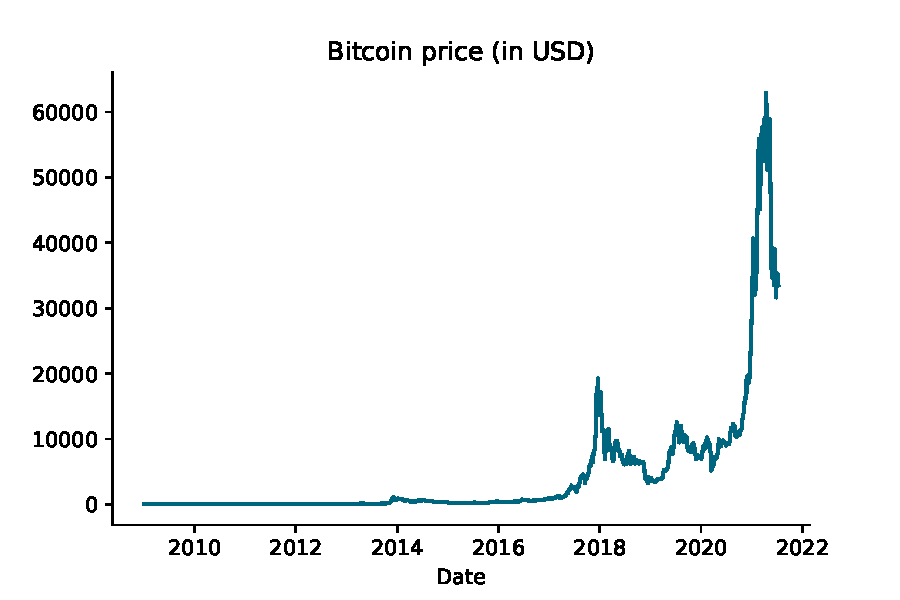
\includegraphics[width=0.42\textwidth]{../../Figures/btc_price}
      \label{sub:QQplot_gamma}
       
                         }
                         \hskip1em
    \subfloat[]{
      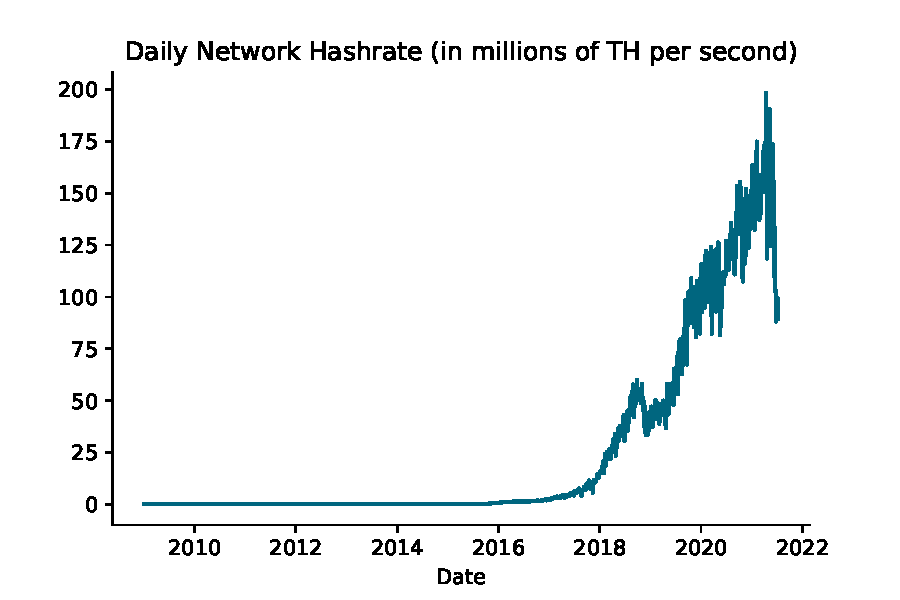
\includegraphics[width=0.42\textwidth]{../../Figures/btc_hahsrate}
      \label{sub:QQplot_weib}
                         }
                         \hskip1em
    \subfloat[]{
      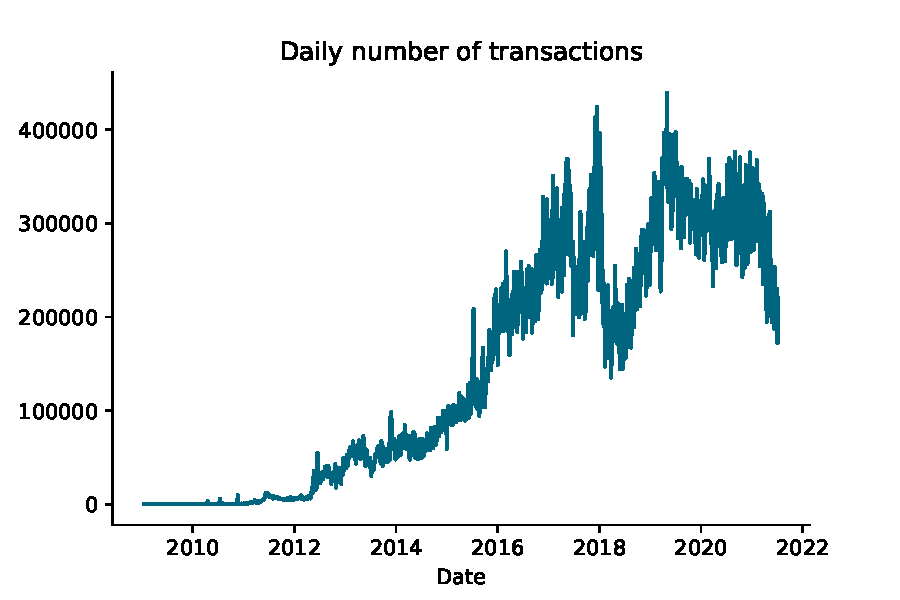
\includegraphics[width=0.42\textwidth]{../../Figures/btc_n_transaction}
      \label{sub:QQplot_lnorm}
                         }
    \subfloat[]{
      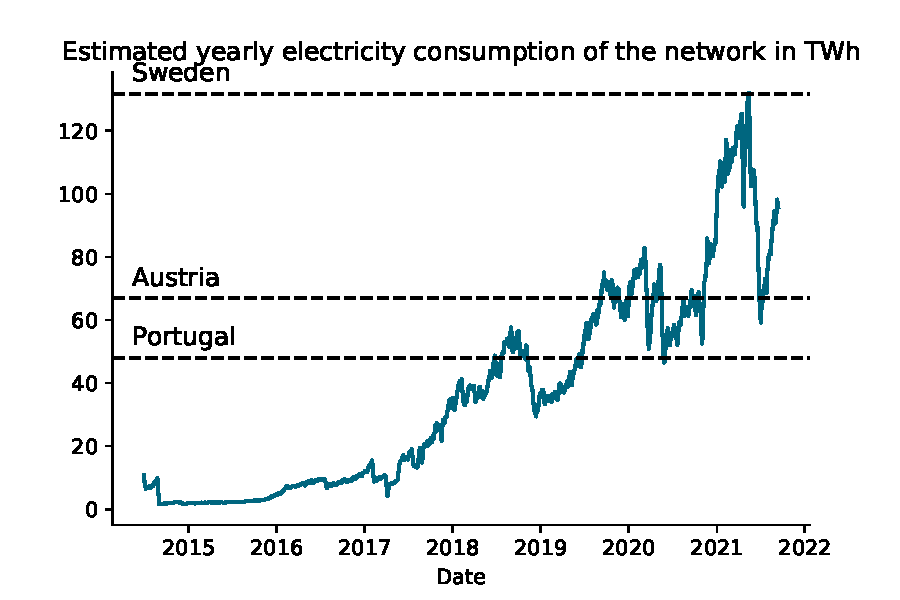
\includegraphics[width=0.42\textwidth]{../../Figures/btc_elec_conso}
      \label{sub:QQplot_pareto}
                         }
    % \caption{Quantile-quantile plots associated to the gamma, Weibull, lognormal and Pareto models fitted to the danish fire insurance loss data using maximum likelihood estimation.}
    % \label{fig:qqplot_weib_lnorm}
  \end{center}
\end{figure}
\blfootnote{\tiny Sources: \url{https://www.blockchain.com/} $\&$ \url{https://cbeci.org/}}
\end{frame}
\begin{frame}{Decentralized finance}
DeFi extends the Bitcoin promises to more complex financial operations 
\begin{itemize}
  \item Collateralized lending
  \item Decentralized Exchange Platform\blfootnote{\url{https://uniswap.org/}}
  \item Tokenized assets
  % \item Fundraising vehicle (ICO, STO, ...)
\end{itemize}
\vspace{0.3cm}
Thanks to Smart Contract on the Ethereum blockchain.
\vspace{0.3cm}
\scriptsize
\begin{thebibliography}{1}

\bibitem{werner2021sok}
S.~M. Werner, D.~Perez, L.~Gudgeon, A.~Klages-Mundt, D.~Harz, and W.~J.
  Knottenbelt, ``Sok: Decentralized finance (defi),'' 2021.

\end{thebibliography}

\end{frame}

\begin{frame}{Decentralized Exchange platforms}
\begin{tcolorbox}[enhanced,drop shadow, title= Centralized Exchange]
Binance, Coinbase, Kraken,...
\begin{itemize}
  \item[$\Rightarrow$] Order book
\end{itemize}
\end{tcolorbox}
\begin{tcolorbox}[enhanced,drop shadow, title= Decentralized Exchange]
Exchange where you trade one token for another through a smart contract on the Ethereum blockchain (ETH).
\begin{itemize}
  \item[$\Rightarrow$] Automated Market Makers (AMM) and Liquidity Providers (LPs)
\end{itemize}
\end{tcolorbox}

 \end{frame}
 \begin{frame}{Order book}
 \begin{columns}
    \column{0.5\textwidth}
    \begin{table}
      \centering
      \caption{Buy Orders}
      \begin{tabular}{ccc}
        \toprule
        Price & Quantity & Total \\
        \midrule
        9,950 & 10 & 99,500 \\
        9,900 & 5 & 49,500 \\
        \bottomrule
      \end{tabular}
    \end{table}
    
    \column{0.5\textwidth}
    \begin{table}
      \centering
      \caption{Sell Orders}
      \begin{tabular}{ccc}
        \toprule
        Price & Quantity & Total \\
        \midrule
        10,100 & 2 & 20,200 \\
        10,200 & 15 & 153,000 \\
        \bottomrule
      \end{tabular}
    \end{table}
  \end{columns}
  and a market maker in the middle to offer liquidity...
  \pause
  \begin{itemize}
  \item[\danger] Lots of transaction must be issued
  \begin{itemize}
  \item[$\hookrightarrow$] Slow (10-15 txs/s)
  \item[$\hookrightarrow$] Expensive (gas fees)
\end{itemize}
\end{itemize}
  
 \end{frame}

\begin{frame}{Automated Market Makers (AMM)}
\begin{columns}
\column{0.5\textwidth}
\footnotesize
A blockchain requires an algorithm $\Rightarrow$ AMM
\begin{itemize}
  \item Exchange one token against another, usually Crypto/Stable Coins

  \item Constant Function Market Makers
  \item Liquidity Providers
  \end{itemize}
  \column{0.5\textwidth}
  \begin{center}

\includegraphics[width=0.6\textwidth]{../../Figures/DALL-E/AMM_BTC_AUSD.png}
\end{center}
  \end{columns}
    \begin{tcolorbox}[enhanced,drop shadow, title=Stable Coin]
    A bridge from fiat to crypto currency
    \begin{itemize}
      \item Fiat-Collateralized Stablecoins (e.g. USDC backed by one USD)
      \item Crypto-Collateralized Stablecoins (e.g. DAI backed by crypto locked in a smart contract)
    \end{itemize}
\end{tcolorbox}

\end{frame}
\begin{frame}{Constant Product Market Maker}
\footnotesize
Let $k$ be a constant such that 
$$
x\cdot y =k,
$$
\begin{itemize}
  \item $x$ is the amount of token $X$
  \item $y$ is the amount of token $Y$
\end{itemize}
    \begin{tcolorbox}[enhanced,drop shadow, title=Example]
    \footnotesize
    ETH$/$DAI Constant Product Market Maker
    \begin{itemize}
      \item Say that the price for one ETH is $P=\$500$
      \item A first LP provides $20$ ETH plus $10,000$ DAI which sets 
      $$k = 20,000$$
      \item The liquidity provided is measured by 
      $$
      L = \sqrt{x\cdot y} \approx 447\text{ (geometric mean)}
      $$
    \end{itemize}
\end{tcolorbox}

\end{frame}
\begin{frame}{Trade on a curve}
\begin{figure}[!ht]
    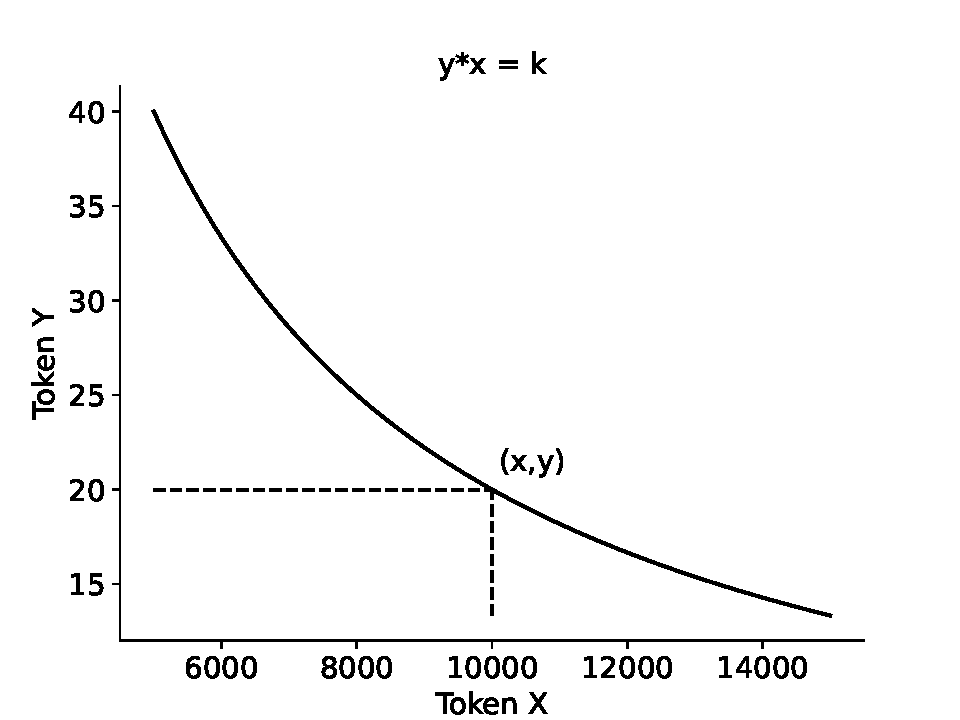
\includegraphics[width = 0.7\textwidth]{../../Figures/AMM_initial.pdf}
    % \captionsetup{width=0.2\textwidth}
    \centering
    % \caption{A block that has not been mined yet.}
    \label{fig:AMM_initial}
\end{figure}
\blfootnote{\tiny The pool never runs out of $X$ nor $Y$}
\end{frame}
\begin{frame}{Swap $X$ for $Y$}
\footnotesize
Acquire $dy$ of token $Y$, then deposit $dx$ that solves
$$
(x+dx)(y-dy) = k\Leftrightarrow dx = \frac{x\cdot dy}{y-dy}
$$
and pay a fee $\alpha \cdot dx$ to the LPs.
\begin{itemize}
  \item[$\Rightarrow$] Price of $Y$ rise in the pool
\end{itemize}
\begin{tcolorbox}[enhanced,drop shadow, title=Example]
    \footnotesize
    Arbitrageur takes $2$ ETH then deposits
    $$
    dx = 1,111 
    $$
    and give out $0.3\cdot 1,111 = 333$ worth of fees
    \begin{itemize}
      \item The price of ETH in the pool rises to 
      $$
      \frac{x+dx}{y-dy} = \$ 617.
      $$
    \end{itemize}
\end{tcolorbox}
\end{frame}
\begin{frame}{Trade on a curve}
\begin{figure}[!ht]
    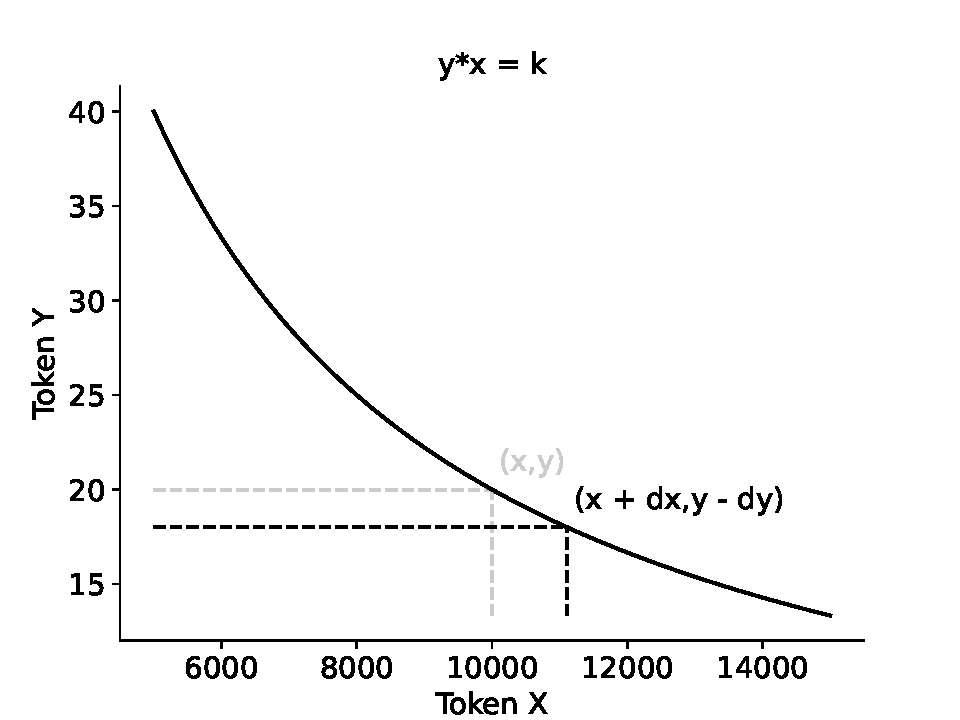
\includegraphics[width = 0.7\textwidth]{../../Figures/AMM_after_swap.pdf}
    % \captionsetup{width=0.2\textwidth}
    \centering
    % \caption{A block that has not been mined yet.}
    \label{fig:AMM_after_swap}
\end{figure}
\end{frame}
\begin{frame}{Add Liquidity}
\footnotesize
Another LP provides $dx$ of token $X$ and thus $dy=\frac{y}{x}dx$ (the price must not change)
\begin{itemize}
\item New level $k' = (x+dx)(y+dy)$
\item Liquidity rises $L' = \sqrt{x\cdot y} + \sqrt{dx\cdot dy}$
\item LPs are weighted according to the liquidity they provide
\item Fees are distributed according to these weights
\end{itemize}
\begin{tcolorbox}[enhanced,drop shadow, title=Example]
    \footnotesize
    New LP deposits $\$5,000$ worth of tokens to the pool then  
    \begin{itemize}
      \item $dx = 2,500$
      \item $dy = 5$
      \item $k' = 312,500$
      \item $L'\approx 559$
    \end{itemize}
    The weights are 
    $$
    \frac{L}{L'} = 0.8\text{ and }\frac{L'-L}{L'} = 0.2.
    $$
\end{tcolorbox}    
\end{frame}
\begin{frame}{Trade on a new curve}
\begin{figure}[!ht]
    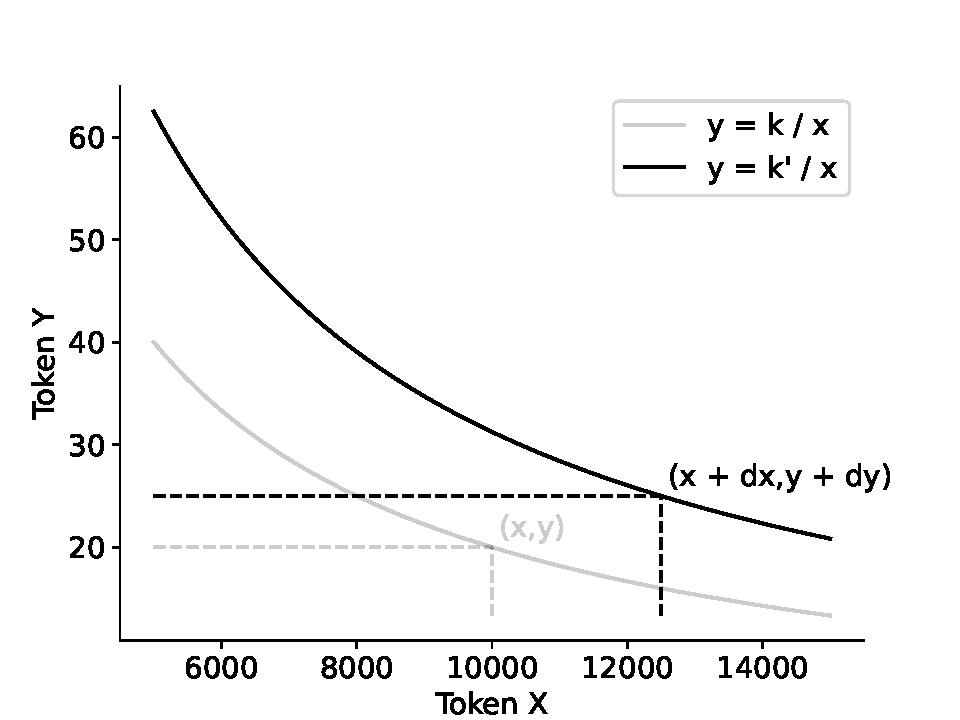
\includegraphics[width = 0.7\textwidth]{../../Figures/AMM_after_drop.pdf}
    % \captionsetup{width=0.2\textwidth}
    \centering
    % \caption{A block that has not been mined yet.}
    \label{fig:AMM_after_drop}
\end{figure}
\end{frame}
\begin{frame}{Flaws of AMM based DEXs}


\begin{itemize}
  \item Price Slippage
  \item Divergent (or impermanent loss)
\end{itemize}

\end{frame}
\begin{frame}{Slippage}
Large trade when using CFMM yields price fluctuations
\begin{itemize}
  \item Many transaction are submitted at the same time
  \begin{itemize}
  \item[$\hookrightarrow$] expected price $\neq$ spot
  \end{itemize}
\end{itemize}
\begin{tcolorbox}[enhanced,drop shadow, title=Sandwich attack]
    \footnotesize
    Validating nodes are aware of pending transaction
    \begin{enumerate}
      \item Find a transaction with high traded volume
      \item Front run that transaction to buy low and/or sell high
    \end{enumerate}
\end{tcolorbox}
\tiny
\begin{thebibliography}{10}

\bibitem{Park2023}
A.~Park, ``The conceptual flaws of decentralized automated market making,''
  {\em Management Science}, vol.~69, pp.~6731--6751, Nov. 2023.



\end{thebibliography}
\end{frame}
\begin{frame}{Impermanent loss}
\begin{center}
Holding tokens VS Locking Tokens in a Smart Contract
\end{center}
\vspace{1cm}
\small
\begin{enumerate}
  \item Liquidity providers deposit pairs of assets 
  \item Trade occurs, the initial ratio of tokens change
  \item LP withdraws $\Rightarrow$ less of the asset that appreciated in value
  \item Divergent loss due to the spread between the initial and current ratio of token that set the price. 
\end{enumerate}

\end{frame}
\begin{frame}{Impermanent Loss}
\footnotesize
The price of $Y$ in the pool is given by 
$$
P = \frac{x}{y},
$$
in terms of token $X$.
\begin{itemize}
  \item Price of $Y$ becomes $P'>P$ on another trading venue then arbitrageurs wish to find
  $$
  \underset{0<dy <y}{\text{argmax }}dy\cdot P' - dx\cdot (1+\alpha) =\underset{0<dy <y}{\text{argmax }}dy\cdot P' - \frac{x\cdot dy}{y-dy}(1+\alpha) 
  $$
  \item We have 
  $$
  dy^\ast = y - \sqrt{\frac{k(1+\alpha)}{P'}}
  $$
  \item The arbitrageurs profit is 
  $$
  dy^\ast\cdot P' -  dx^\ast (1+\alpha)
  $$
  \item It coincides with the impermanent loss of the LPs
  $$
  y\cdot P' + x - [(y-dy^\ast)\cdot P' + x + dx^\ast(1+\alpha)]
  $$
\end{itemize}
\end{frame}
\begin{frame}{Impermanent Loss}
The loss becomes permanent if 
\begin{itemize}
  \item The LPs withdraw their funds
  \item The price of the asset is not mean reverting
\end{itemize}
\begin{tcolorbox}[enhanced,drop shadow, title=Example]
    Suppose that $P' = \$550$ and $\alpha = 0$ then 
    \begin{itemize}
      \item $dy^\ast = 0.93$
      \item The impermanent loss is then $dy^\ast\cdot P' -\frac{xdy^\ast}{y - dy^\ast} = \$23$
    \end{itemize}
\end{tcolorbox}
\end{frame}

\begin{frame}{Impermanent loss}
\footnotesize
The trading fee allows a pool to mitigate the impermanent loss
\begin{figure}[!ht]
    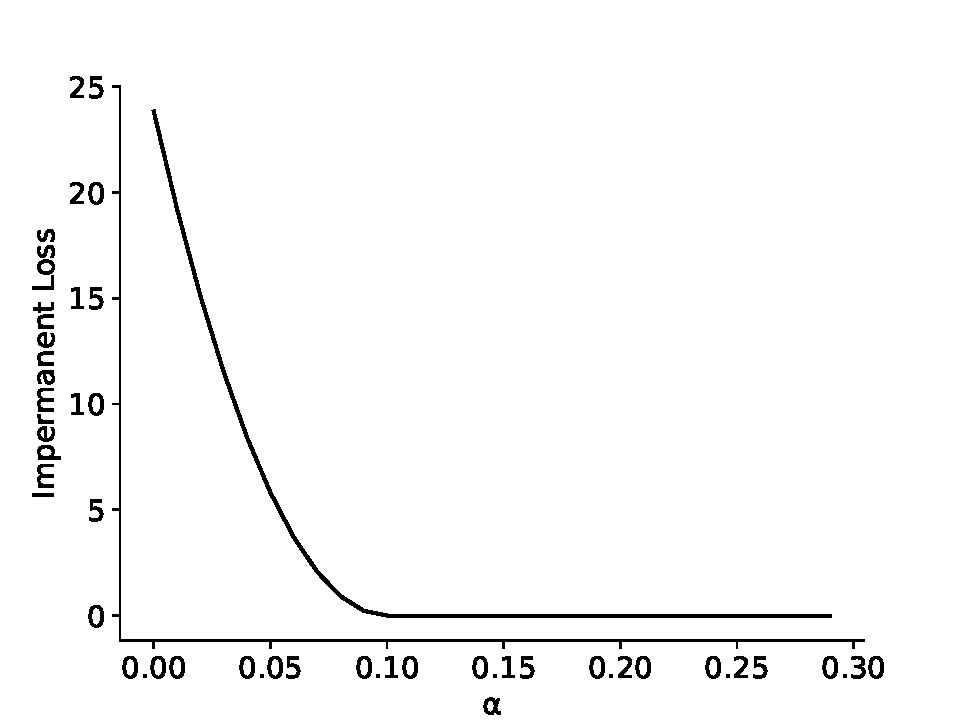
\includegraphics[width = 0.5\textwidth]{../../Figures/imp_loss.pdf}
    % \captionsetup{width=0.2\textwidth}
    \centering
    % \caption{A block that has not been mined yet.}
    \label{fig:imp_loss}
\end{figure}
But high trading fees makes the DEX unattractive... UNISWAP V3 and concentrated liquidity\blfootnote{\url{https://uniswap.org/whitepaper-v3.pdf}}.
\end{frame}

\begin{frame}{Decentralized insurance}
\begin{tcolorbox}[enhanced,drop shadow, title=Parametric insurance]
    Compensation if a measurable quantity reaches a threshold 
\end{tcolorbox}
\begin{itemize}
  \item Example: Flight delay insurance
  \begin{itemize}
    \item \url{https://etherscan.io/address/0xdc3d8fc2c41781b0259175bdc19516f7da11cba7}
  \end{itemize}
  \item Use smart contract and off-chain data through oracles
  \item Transparent and automatic
\end{itemize}
\end{frame}


\begin{frame}{Blockchain as a research topic}
\begin{itemize}
  \item Computer science
  \begin{itemize}
  \item Peer-to-peer networks and consensus algorithm
  \item Cryptography and security
  \end{itemize}
  \item Economics  
  \begin{itemize}
  \item Game theory to study the incentive mechanism at play
  \item Nature of the cryptoassets
  \end{itemize}
  \item Operations research  
  \begin{itemize}
  \item Optimization of complex system
  \end{itemize}
  \item Financial math  
  \begin{itemize}
  \item Valuation models for cryptoassets
  \end{itemize}
  \item Machine learning and statistics  
  \begin{itemize}
  \item Open data
  \item Interaction between blockchain users
  \item (Social) network analysis
  \item Clustering of public keys and addresses in the bitcoin blockchain.
  \end{itemize}
\end{itemize}

\end{frame}
\appendix
\begin{frame}{Byzantine General problem}
    $n$ generals must agree on a common battle plan, to either 
    \begin{itemize}
    \item Attack (A) 
    \item Retreat (R)
  \end{itemize}
\begin{tcolorbox}[enhanced,drop shadow, title=Problem]
There are $m<n$ traitors among the generals
\end{tcolorbox}
\begin{enumerate}
\item message $m(i,j)$ is sent to general $j$ by general $i$ 
\item Consensus is reached as general $j$ applies 
$$
f(\{m(i,j);\text{ }i = 1,\ldots,n\}) = \begin{cases}
A,& \text{if }\sum_{i = 1}^n\mathbb{I}_{m(i,j) =A} >n/2,\\
R, &\text{else}.
\end{cases}
$$
\end{enumerate}
\end{frame}
\begin{frame}[plain]
\begin{figure}[!ht]
 \begin{center}
 \subfloat[No traitor]{
\begin{tikzpicture}[->, >=stealth', auto, semithick, node distance=2cm]
\tikzstyle{every state}=[fill=white,draw=black,thick,text=black,scale=0.8]
\node[state]    (1)                     {$G_1$};
\node[state]    (2)[below of=1]   {$G_2$};
\node[state]    (3)[below of=2]   {$G_3$};
\node[state]    (4)[below of=3]   {$G_4$};
\node[state]    (5)[below of=4]   {$G_5$};
\node[draw] (6) [right of=1]   { \footnotesize$f({A,R,R,A,A}) = A$};
\node[draw] (7) [right of=2]   { \footnotesize$f({A,R,R,A,A}) = A$};
\node[draw] (8) [right of=3]   { \footnotesize$f({A,R,R,A,A}) = A$};
\node[draw] (9) [right of=
4]   { \footnotesize$f({A,R,R,A,A}) = A$};
\node[draw] (10) [right of=5]   { \footnotesize$f({A,R,R,A,A}) = A$};
\path
(1) edge[bend left]     node{ A}     (2)
(2) edge[bend left]     node{ R}      (1)
(2) edge[bend left]     node{ R}      (3)
(3) edge[bend left]     node{ R}      (2)
(3) edge[bend left]     node{ R}      (4)
(4) edge[bend left]     node{ A}      (3)
(4) edge[bend left]     node{ A}      (5)
(5) edge[bend left]     node{ A}      (4)
;
\path
(1) edge     (6)
(2) edge     (7)
(3) edge     (8)
(4) edge     (9)
(5) edge     (10)
;
\end{tikzpicture}
\label{fig:no_traitor}}
\hskip2em
 \subfloat[One traitor]{
\begin{tikzpicture}[->, >=stealth', auto, semithick, node distance=2cm]
\tikzstyle{every state}=[fill=white,draw=black,thick,text=black,scale=0.8]
\node[state]    (1)                     {$G_1$};
\node[state]    (2)[below of=1]   {$G_2$};
\node[state]    (3)[below of=2]   {$G_3$};
\node[state]    (4)[below of=3]   {\color{red}$G_4$};
\node[state]    (5)[below of=4]   {$G_5$};
\node[draw] (6) [right of=1]   { \footnotesize$f({A,R,R,R,A}) = R$};
\node[draw] (7) [right of=2]   { \footnotesize$f({A,R,R,R,A}) = R$};
\node[draw] (8) [right of=3]   { \footnotesize$f({A,R,R,R,A}) = R$};
\node[draw] (9) [right of=
4]   { \footnotesize$f({A,R,R,?,A}) = ?$};
\node[draw] (10) [right of=5]   { \footnotesize$f({A,R,R,A,A}) = A$};
\path
(1) edge[bend left]     node{ A}     (2)
(2) edge[bend left]     node{ R}      (1)
(2) edge[bend left]     node{ R}      (3)
(3) edge[bend left]     node{ R}      (2)
(3) edge[bend left]     node{ R}      (4)
(4) edge[bend left]     node{ \color{red}R}      (3)
(4) edge[bend left]     node{ \color{red}A}      (5)
(5) edge[bend left]     node{ A}      (4)
;
\path
(1) edge     (6)
(2) edge     (7)
(3) edge     (8)
(4) edge     (9)
(5) edge     (10)
;
\end{tikzpicture}
\label{fig:_one_traitor}}
\end{center}
\caption{Majority vote with or without a traitor}
\label{fig:majority_vote}
\end{figure}
\end{frame}
\begin{frame}{Commanders and Lieutenants}
One general is the commander while the others are the lieutenants
\begin{tcolorbox}[enhanced,drop shadow, title=Objective]
Design an algorithm so that the following conditions are met:
\begin{itemize}
  \item[C1] All the loyal lieutenants obey the same order
  \item[C2] If the commanding general is loyal, then  every loyal lieutenants obey the order he sends
\end{itemize}
\end{tcolorbox}
\begin{tcolorbox}[enhanced,drop shadow, title=Byzantine Fault Tolerance Theorem (Lamport et al.)]
There are no solution to the Byzantine General problem for $n<3m+1$ generals, where $m$ is the number of traitors.
\end{tcolorbox}
\end{frame}
\begin{frame}[plain]
\begin{figure}[!ht]
 \begin{center}
 \subfloat[Commander is loyal]{
\begin{tikzpicture}[->, >=stealth', auto, semithick, node distance=4cm]
\tikzstyle{every state}=[fill=white,draw=black,thick,text=black,scale=0.8]
\node[state]    (1)               {C};
\node[state]    (2)[below left of=1]   {L1};
\node[state]    (3)[below right of=1]   {\begin{color}{red}L2 \end{color}};
\path
(1) edge[bend left]     node{A}     (3)
(1) edge[bend right, above]     node{A}      (2)
(2) edge[bend left]     node{A}      (3)
(3) edge[bend left]     node{R}      (2)
% (3) edge[bend left]     node{R}      (4)
% (4) edge[bend left]     node{A}      (3)
% (4) edge[bend left]     node{A}      (5)
% (5) edge[bend left]     node{A}      (4)
;
\end{tikzpicture}
\label{fig:commander_loyal}}
\hskip2em
\subfloat[Commander is a traitor]{
\begin{tikzpicture}[->, >=stealth', auto, semithick, node distance=4cm]
\tikzstyle{every state}=[fill=white,draw=black,thick,text=black,scale=0.8]
\node[state]    (1)               {\begin{color}{red}C \end{color}};
\node[state]    (2)[below left of=1]   {L1};
\node[state]    (3)[below right of=1]   {L2};
\path
(1) edge[bend left, above]     node{A}     (3)
(1) edge[bend right, above]     node{R}      (2)
(2) edge[bend left]     node{R}      (3)
(3) edge[bend left]     node{A}      (2)
% (3) edge[bend left]     node{R}      (4)
% (4) edge[bend left]     node{A}      (3)
% (4) edge[bend left]     node{A}      (5)
% (5) edge[bend left]     node{A}      (4)
;
\end{tikzpicture}
\label{fig:commander_traitor}}
\end{center}
\caption{Majority vote with or without a traitor}
\label{fig:majority_vote}
\end{figure}
\end{frame}
% \begin{frame}[plain]
% \begin{algorithm}[H]
% \caption{The Oral message algorithm $\text{OM}(m)$}\label{alg:om}
% \begin{algorithmic}
% \If{$m=0$};
% \For{$i =1 \to n-1$} 
% \State Commander sends $v_i = v$ to lieutenant $i$ 
% \State Lieutenant $i$ set their value to $v$
% \EndFor
% \EndIf
% \If{$m>0$};
% \For{$i =1 \to n-1$} 
% \State Commander sends $v_i$ to lieutenant $i$ 
% \State Lieutenant $i$ uses OM(m-1) to communicate $v_i$ to the $n-2$ lieutenants
% \EndFor
% \For{$i =1 \to n-1$} 
% \State Lieutenant $i$ set their value to $f(v_1, \ldots, v_{n-1})$
% \EndFor
% \EndIf
% \end{algorithmic}
% \end{algorithm}
% \end{frame}
\begin{frame}{$n = 4$ and $m = 1$: Step 1}
\begin{figure}[!ht]
 \begin{center}
 \subfloat[Commander is loyal]{
\begin{tikzpicture}[->, >=stealth', auto, semithick, node distance=4cm]
\tikzstyle{every state}=[fill=white,draw=black,thick,text=black,scale=0.8]
\node[state]    (1)               {C};
\node[state]    (2)[below left of=1]   {L1};
\node[state]    (3)[below of=1]   {L2};
\node[state]    (4)[below right of=1]   {\begin{color}{red}L3 \end{color}};
\path
(1) edge[bend right]     node{A}     (2)
(1) edge[bend left]     node{A}      (4)
(1) edge     node{A}      (3)
% (2) edge[bend right, below]     node{A}      (3)
% (3) edge[bend right, above]     node{A}      (2)
% (4) edge[bend right, above]     node{R}      (3)
% (3) edge[bend right, below]     node{A}      (4)
;
\end{tikzpicture}
\label{fig:commander_loyal_om}}
\hskip2em
\subfloat[Commander is a traitor]{
\begin{tikzpicture}[->, >=stealth', auto, semithick, node distance=4cm]
\tikzstyle{every state}=[fill=white,draw=black,thick,text=black,scale=0.8]
\node[state]    (1)               {\begin{color}{red}C \end{color}};
\node[state]    (2)[below left of=1]   {L1};
\node[state]    (3)[below of=1]   {L2};
\node[state]    (4)[below right of=1]   {L3};
\path
(1) edge[bend right]     node{A}     (2)
(1) edge[bend left]     node{R}      (4)
(1) edge     node{R}      (3)
% (2) edge[bend right, below]     node{A}      (3)
% (3) edge[bend right, above]     node{R}      (2)
% (4) edge[bend right, above]     node{R}      (3)
% (3) edge[bend right, below]     node{R}      (4)
;
\end{tikzpicture}
\label{fig:commander_traitor_om}}
\end{center}
\caption{Illustration of the \text{OM}(m) algorithm in the case where $n = 4$ and $m=1$.}
\label{fig:OM_algorithm_illustration}
\end{figure}
\end{frame}
\begin{frame}{$n = 4$ and $m = 1$: Step 2}
\begin{figure}[!ht]
 \begin{center}
 \subfloat[Commander is loyal]{
\begin{tikzpicture}[->, >=stealth', auto, semithick, node distance=4cm]
\tikzstyle{every state}=[fill=white,draw=black,thick,text=black,scale=0.8]
\node[state]    (1)               {C};
\node[state]    (2)[below left of=1]   {L1};
\node[state]    (3)[below of=1]   {L2};
\node[state]    (4)[below right of=1]   {\begin{color}{red}L3 \end{color}};
\path
(1) edge[bend right]     node{A}     (2)
(1) edge[bend left]     node{A}      (4)
(1) edge     node{A}      (3)
(2) edge[bend right, below]     node{A}      (3)
(3) edge[bend right, above]     node{A}      (2)
(4) edge[bend right, above]     node{R}      (3)
(3) edge[bend right, below]     node{A}      (4)
;
\end{tikzpicture}
\label{fig:commander_loyal_om}}
\hskip2em
\subfloat[Commander is a traitor]{
\begin{tikzpicture}[->, >=stealth', auto, semithick, node distance=4cm]
\tikzstyle{every state}=[fill=white,draw=black,thick,text=black,scale=0.8]
\node[state]    (1)               {\begin{color}{red}C \end{color}};
\node[state]    (2)[below left of=1]   {L1};
\node[state]    (3)[below of=1]   {L2};
\node[state]    (4)[below right of=1]   {L3};
\path
(1) edge[bend right]     node{A}     (2)
(1) edge[bend left]     node{R}      (4)
(1) edge     node{R}      (3)
(2) edge[bend right, below]     node{A}      (3)
(3) edge[bend right, above]     node{R}      (2)
(4) edge[bend right, above]     node{R}      (3)
(3) edge[bend right, below]     node{R}      (4)
;
\end{tikzpicture}
\label{fig:commander_traitor_om}}
\end{center}
\caption{Illustration of the \text{OM}(m) algorithm in the case where $n = 4$ and $m=1$.}
\label{fig:OM_algorithm_illustration}
\end{figure}
\end{frame}
\begin{frame}{$n = 4$ and $m = 1$: Step 3}
\begin{figure}[!ht]
 \begin{center}
 \subfloat[Commander is loyal, C1 and C2]{
\begin{tikzpicture}[->, >=stealth', auto, semithick, node distance=4cm]
\tikzstyle{every state}=[fill=white,draw=black,thick,text=black,scale=0.78]
\node[state]    (1)               {C};
\node[state]    (2)[below left of=1]   {L1};
\node[state]    (3)[below of=1]   {L2};
\node[state]    (4)[below right of=1]   {\begin{color}{red}L3 \end{color}};

\path
(1) edge[bend right]     node{A}     (2)
(1) edge[bend left]     node{A}      (4)
(1) edge     node{A}      (3)
(2) edge[bend right, below]     node{A}      (3)
(3) edge[bend right, above]     node{A}      (2)
(4) edge[bend right, above]     node{R}      (3)
(3) edge[bend right, below]     node{A}      (4)
(2) edge[loop below] node{\tiny f(A,A,R)=A } (2)
(3) edge[loop below] node{\tiny f(A,A,R)=A } (3)
;
\end{tikzpicture}
\label{fig:commander_loyal_om}}
\hskip1em
\subfloat[Commander is a traitor, C1]{
\begin{tikzpicture}[->, >=stealth', auto, semithick, node distance=4cm]
\tikzstyle{every state}=[fill=white,draw=black,thick,text=black,scale=0.78]
\node[state]    (1)               {\begin{color}{red}C \end{color}};
\node[state]    (2)[below left of=1]   {L1};
\node[state]    (3)[below of=1]   {L2};
\node[state]    (4)[below right of=1]   {L3};
\path
(1) edge[bend right]     node{A}     (2)
(1) edge[bend left]     node{R}      (4)
(1) edge     node{R}      (3)
(2) edge[bend right, below]     node{A}      (3)
(3) edge[bend right, above]     node{R}      (2)
(4) edge[bend right, above]     node{R}      (3)
(3) edge[bend right, below]     node{R}      (4)
(2) edge[loop below] node{\tiny f(A,R,R)=R } (2)
(3) edge[loop below] node{\tiny f(A,R,R)=R } (3)
;
;
\end{tikzpicture}
\label{fig:commander_traitor_om}}
\end{center}
\caption{Illustration of the \text{OM}(m) algorithm in the case where $n = 4$ and $m=1$.}
\label{fig:OM_algorithm_illustration}
\end{figure}
\end{frame}
\begin{frame}{The problem with majority vote}
The OM algorithm requires to send $n^{m+1}$
\begin{itemize}
  \item[\danger] Communication overhead
  \item[\danger] Denial of service
\end{itemize}
\begin{tcolorbox}[enhanced,drop shadow, title=Solution]
Leader based protocols!
\end{tcolorbox}
\end{frame}



\end{document}
